\documentclass[12pt]{article}
\usepackage{sbc-template}
\usepackage[]{graphicx,url}
\usepackage{mathtools}
\usepackage[brazil]{babel}
\usepackage[utf8]{inputenc}

\usepackage[autostyle]{csquotes}

\usepackage{multirow}
\usepackage[table,xcdraw]{xcolor}
\usepackage[colorinlistoftodos]{todonotes}
\usepackage[colorlinks=true, allcolors=blue]{hyperref}

\usepackage{subfigure}

\sloppy

\title{Sistema de Recomendação Baseado em Confiança para Promover a Colaboração em Redes de Pesquisa Científica}

\author{João Pedro R. D. Saldanha\inst{1}, Alexandre Zamberlan\inst{1}, Fernando Prass\inst{1}}


\address{Ciência da Computação -- Universidade Franciscana (UFN)\\
  Rua dos Andradas, 1614  -- 97010-032  -- Santa Maria -- RS -- Brasil
\email{\{joao.pedro,alexz,fernando.prass\}@ufn.edu.br}
}

\begin{document} 

\maketitle

\begin{abstract}
  This paper presents a proposal for building a recommender system that promotes collaboration between researchers in a publication network. A trust network is abstracted in which researchers are bound by joint publications, which represents a mutual trust statement. Metrics are discussed for  computing trust. An architecture is proposed to improve recommendation quality trough profile analysis.
\end{abstract}

\begin{resumo} 
  Este artigo apresenta a proposta da elaboração de um sistema de recomendações para promover a colaboração entre pesquisadores em uma rede de publicações. É abstraída uma rede de confiança na qual pesquisadores são unidos por publicações em conjunto, que constituem um voto de confiança mútua. São discutidas métricas de computação de confiança. Foi proposta uma arquitetura para melhorar as recomendações por meio de análise de perfil.
\end{resumo}

\section{Introdução}

O universo da pesquisa científica está em constante expansão, tanto no que diz respeito ao conhecimento produzido quanto ao volume de trabalhos e publicações. Estimativas apontavam um valor em torno de 2.5 milhões de artigos científicos publicados por ano em 2015, com um aumento de 5\% ao ano no número de cientistas fazendo publicações \cite{ware2015stm}. Pesquisadores não têm o tempo necessário para analisar todos os estudos relacionados à seus próprios trabalhos, mesmo com plataformas como o Lattes, onde tais trabalhos estão compilados. Trata-se do problema da sobrecarga de informação, que tem crescido na medida em que sistemas digitais vem ganhando cada vez usuários e conteúdo. Outro problema decorrente do crescimento do número de pesquisadores e trabalhos é que muitas vezes os pesquisadores não conhecem outros pesquisadores da área e acabam por perder a oportunidade de colaborações ou troca de ideias. Logo, faz-se necessário a filtragem da informação que chega ao pesquisador para maximizar sua eficiência e evitar tempo perdido. A automação da tarefa de filtragem é feita através de sistemas de recomendação. Utilizando técnicas de mineração de dados e inteligência artificial pode-se oferecer conteúdo mais relevante, aumentando a eficiência do acadêmico. 

A partir do problema da sobrecarga de informações, nos anos 90 iniciou-se a pesquisa na área de filtragem de conteúdo. O ponto de partida foi a observação que as pessoas usam, no dia-a-dia, dicas de outros para tomar decisões. Os primeiros sistemas de recomendação eram algoritmos capazes de analisar tendências dentro de uma  comunidade e então fazer sugestões aos seus membros. Esse método é conhecido como filtragem colaborativa e foi aprimorado desde então, sendo até hoje bastante popular. Além deste, também é bastante difundido o método baseado em conteúdo, no qual novos itens são recomendados baseado no conteúdo consumido pelo usuário no passado \cite{ricci2011introduction}.

Neste trabalho, o foco foi sistema de recomendação guiado por estimativa (ou heurística) de confiança. Confiança é um sentimento que pode ser descrito como o ato de contar com a credibilidade e consistência das ações de um indivíduo. Trata-se de um elemento citado por muitos autores como o mais importante para a construção de uma relação de trabalho positiva, por ser essencial para criticismo construtivo e evolução mútua dentro do processo de pesquisa \cite{bagshaw2007international}. Os dados de analise tem origem na plataforma Lattes. Para a elaboração do sistema proposto, é preciso: estudar funções e aplicações de sistemas de recomendação; modelar a rede de confiança da comunidade científica; estabelecer métricas de confiança para os dados disponíveis; estimar a confiança entre os pesquisadores; pré-selecionar recomendações; filtrar a pré-seleção com a confiança computada. Para solucionar o problema explanado, propõe-se descrever uma rede de colaborações a partir de publicações em conjunto, discutida na Seção~\ref{sect:computing-trust} utilizando técnicas encontradas na literatura para computar a propagação de confiança na rede. A partir disso, é discutida a pré-seleção dos itens com o método baseado em conteúdo (Seção~\ref{sect:pre-selection}), proposta uma arquitetura para o sistema de recomendações (Seção~\ref{sect:arch}).

\section{Revisão Bibliográfica}

Nesta seção, são apresentados os itens que compõem o embasamento teórico usado.

\subsection{Sistemas de Recomendação}

Os itens recomendados pelo Sistema de Recomendação (SR) podem ser os mais variados, sendo que no geral a recomendação é uma tarefa especializada na qual um tipo de item é considerado relevante para um perfil específico de usuário. Logo, a metodologia usada para sua construção, interface de usuário e critério para ordenar os resultados devem ser adaptados às especificidades da tarefa em questão \cite{ricci2011introduction}. 

O resultado obtido por um SR é dependente da realização de uma \textbf{predição}, itens são apresentados ao usuário porque o sistema antecipa que sejam relevantes para ele \cite{ricci2011introduction}. Geralmente na elaboração de sistemas de recomendação lida-se com \textbf{usuários}, denotados por $ u_1, ... u_n \in U $, \textbf{itens}, denotados por $ i_1, ... i_n \in I$  e \textbf{relações}, que associam usuários e itens de diversas maneiras \cite{ekstrand2019recommender}. As associações podem ser representadas por ontologias \cite{primo2006tecnicas} ou no caso de relações entre usuários e itens através de uma matriz de associação $ |U| \times |I| $. Assume-se a existência no mundo real de uma função $ f (u, i) $ que retorne um número real representado a utilidade do item $i$ ao usuário $u$. Em técnicas de filtragem colaborativa, este numero é visto como a avaliação do usuário. A tarefa do SR neste contexto é computar uma função $\hat{f}(u, i)$ que se assemelhe ao máximo à $f$. Assim, é possível realizar a predição de relevância de um grupo de itens para determinado usuário $\hat{f}(u_n, I)$ e recomendar os itens melhores classificados pelo SR, efetivamente filtrando o conteúdo e oferecendo ao usuário uma seleção personalizada de itens \cite{ricci2011introduction}.

A forma mais simples do resultado de um SR é uma lista de itens ordenada de acordo com a preferência do usuário. A satisfação com as recomendações pode ser coletada explicitamente, como por exemplo por meio de avaliações, ou implicitamente com inferências baseadas no comportamento do usuário perante aos itens oferecidos. Para oferecer recomendações, é preciso analisar  uma base de conhecimento, realizar um trabalho de classificação dos itens ofertados e então coletar algum tipo de \textit{feedback} perante o resultado que deve ser usado para aprimorar o sistema \cite{shani2011evaluating}.

Técnicas de filtragem colaborativa analisam o \textbf{perfil} do usuário e sua \textbf{avaliação} dos itens previamente acessados para chegar em recomendações. Procura-se achar um \textit{cluster} de usuários com perfis similares (\textbf{vizinhos}). A ideia é que os itens bem avaliados pelos vizinhos serão também avaliados positivamente pelo usuário alvo, já que os perfis são semelhantes. Um problema encontrado na técnica é o da \textit{primeira avaliação}: quando há um item novo, sem nenhuma avaliação, como saber se determinado usuário irá avaliar positivamente o mesmo? Nenhum de seus vizinhos fez avaliações \cite{ricci2011introduction}. SR baseados em filtragem colaborativa são os mais populares na área e vêm sido pesquisados há mais tempo \cite{ricci2011introduction}. É comum utilizar métodos baseados em vizinhança, nos quais um algoritmo de clusterização tal como o algoritmo \textbf{KNN} (\textit{K-Nearest Neighbours}) é usado para determinar grupos de usuários \cite{da2018desenvolvimento}.

O método baseado em conteúdo parte da ideia de que usuários têm interesse em itens semelhantes àqueles que lhe foram uteis no passado \cite{ricci2011introduction}. No caso, é importante determinar a \textbf{semelhança entre itens} para então recomendar itens semelhantes aos que foram previamente bem avaliados pelo usuário. Nesse método é preciso estabelecer estratégias para descrever itens, bem como para montar o perfil dos usuários descrevendo os tipos de itens que ele tem interesse. Deve ser feito o comparativo dos itens com o perfil do usuário para predizer seu interesse. Geralmente procura-se dividir o universo dos itens, $I$, em categorias: relevantes ou irrelevantes. Para construir a classificação dos itens é possível usar uma série de algoritmos que realizam trabalho de classificação estatística, como por exemplo árvores de decisão. \cite{pazzani2007content}.

Conforme \cite{sinha2001comparing}, estudos indicam que os usuários têm a tendência de valorizar mais as recomendações de amigos do que aquelas feitas por outros usuários com perfil semelhante, porém desconhecidos e a qualidade das recomendações de amigos superam inclusive as feitas por sistemas de recomendação. A partir deste conceito, com a grande aderência de usuários à redes sociais um novo método para a construção de sistemas de recomendação está sendo estudado, trata-se do método baseado em confiança, ou sistema de recomendação social  \cite{ricci2011introduction}. A construção de SR sociais depende do estabelecimento de uma \textbf{rede de confiança}, rede que descreve o nível de confiança entre seus membros. Assim, o usuário recebe recomendações de itens avaliados positivamente por usuários em sua rede de confiança. Estes SR usam o conceito de agregação e dissipação de confiança, ou seja, dado um grupo de usuários $u_1  \dots u_n$, calcular o nível de confiança entre $u_1$ e $u_n$ considerando usuários intermediários $u_2 \dots u_{n-1}$ que possuem alguma relação de confiança, direta ou indireta, com $u_1$ e $u_n$ (\textbf{dissipação}) ou combinar uma série de estimativas de confiança em um valor final (\textbf{agregação}) \cite{victor2011trust}. Um ponto fraco de tais sistemas é que a recomendação é geralmente mais previsível e pode facilmente ser inundada por itens que o usuário já conhece, enquanto técnicas mais usuais de recomendação podem apresentar resultados mais inesperados, mas relevantes ao usuário \cite{sinha2001comparing}.

Métodos híbridos propõem a combinação de mais de um método de recomendação dentro de um sistema. É necessário para complementar técnicas que podem apresentar problemas em determinadas situações ou para oferecer resultados melhores aos usuários. Furlan \cite{da2018desenvolvimento} combinou os métodos baseado em conteúdo e filtragem colaborativa para solucionar o problema da primeira avaliação. Já Massa \cite{massa2004trust} sugere que um método que leve em consideração a confiança entre usuários pode melhorar a performance de sistemas de filtragem colaborativa.

\subsection{Análise de Dados em Redes Sociais}\label{sect:analysis}

Pode-se pensar na rede de colaborações como sendo um grafo, os nodos são pesquisadores e as arestas publicações em conjunto. Além disso uma colaboração em publicações é um voto de confiança entre os pesquisadores envolvidos. A matriz de adjacência pode ser usada para computar a propagação de confiança por meio da rede. A confiança estimada de determinado pesquisador pode levar em consideração o nível de confiança estimado dos pesquisadores que colaboraram com ele. Outro fator que pode ser considerado é a facilidade de colaboração, levando em  consideração “distâncias” na rede: se dois pesquisadores A e B têm laços de confiança com um intermediário C, a colaboração entre A e B tende a ser mais fácil do que se houvesse mais intermediários na rede.

O algoritmo PageRank \cite{page1999pagerank} foi inspirado em parte por estudos realizados em redes de citações acadêmicas, nas quais a relevância de um artigo era descrita por contagem de citações, por exemplo. Trata-se de um método para computar um \textit{ranking}  global de citações, pensado para obter a importância das páginas web. O \textit{ranking} $R$ de uma página é definido como a soma dos \textit{rankings} das páginas que oferecem \textit{links} para ela, ponderada pelo total de \textit{links} encontrados nas páginas. O algoritmo funciona da seguinte forma: é definido para cada página $u$ um conjunto $F_u$ de páginas as quais $u$ referencia e um conjunto $B_u$ de páginas que fazem referência à $u$. Sendo $\hat{A}$ a matriz de adjacência da web, tal que 

\begin{equation} \label{eqn:adjacency-matrix}
   \hat{A}_{i,j} =
    \begin{cases}
      1       & \quad \text{se } \text{ há links de i para j}\\
      0       & \quad \text{se } \text{ não há links de i para j}
    \end{cases}
\end{equation}

A matriz $A$ deve ser obtida dividindo todas as linhas de $\hat{A}$ por $|F_u|$ (o grau do nodo $u$). Assim, PageRank pode ser definido como $R = c(AR + E)$, sendo $c$ um fator de normalização.

Quando ocorrem ciclos no fluxo de referência, nos quais duas páginas se referenciam mutuamente e não fazem referência a nenhuma outra página, pode ocorrer o chamado \textit{rank sink}: referências exteriores injetam \textit{ranking} no ciclo, fazendo com que páginas do ciclo acumulem pontuação, porém sem distribuição. Para solucionar, foi introduzido o vetor $E$, que no modelo de PageRank é o conceito de um \textit{random surfer}, ou seja, uma heurística representando a probabilidade de um usuário da internet aleatoriamente mudar a página, sem seguir nenhum de seus \textit{links} \cite{page1999pagerank}.

Já a centralidade è uma métrica da teoria dos grafos usada para representar a importância de um nodo na rede. Centralidade de grau è definida como o numero de arestas com as quais um nodo se conecta. A métrica de centralidade apresentada em \cite{opsahl2010node} se encaixa particularmente bem em casos nos quais o peso da aresta representa a força da conexão, tal qual o problema proposto neste trabalho, por incorporar simultaneamente o grau (número de conexões) e a força (os pesos de cada conexão) dos nodos. O peso pode ser a soma das relevâncias das obras publicadas em conjunto entre os pesquisadores. A fórmula proposta pelos autores faz isso definindo um parâmetro $\alpha$ para ajustar a importância de grau e força:

\begin{equation} \label{eqn:centrality} 
 C_D ^{w \alpha} (i) = k_i \times \left( \frac {s_i} {k_i} \right) ^{\alpha} = k_i ^{1 - \alpha} \times s _i ^{\alpha}
\end{equation}

No contexto de distância, o algoritmo de Dijikstra \cite{dijkstra1959note} é definido para calcular distâncias em redes nas quais os pesos representam o custo de travessia. O trabalho de Opsahl e Skvoretz \cite{opsahl2010node} é definido em redes onde os pesos representam força dos laços, então os autores sugerem que os pesos devem ser invertidos. Além disso, o objetivo do trabalho é considerar também o número de nós intermediários, então os autores propõem novamente o uso de um parâmetro de ajuste, $\alpha$, que controla o quão importante considera-se o número de nodos intermediários e a força das conexões.

\begin{equation} \label{eqn:distance}
  d^{w\alpha}(i, j) = min \left( \frac{1}{ \left( w_{ih}^{\alpha} \right) } + \dots + \frac{1}{ \left( w_{hj}^{\alpha} \right) }  \right) 
\end{equation}

Frequentemente na análise de dados é necessário o uso de clusterização. O algoritmo MeanShift é indicado para dados nos quais se espera muitos \textit{clusters} distintos e de tamanhos variáveis \cite{scikit-learn}. A implementação é descrita como uma busca por centróides baseada em grafo de vizinhos mais próximos. O parâmetro \textit{bandwidth} é usado como estimativa para o tamanho dos \textit{clusters}.

\subsection{Trabalhos Correlatos}

Os trabalhos correlatos foram escolhidos utilizando como critério a contemporaneidade e semelhança com o presente trabalho.

No trabalho de \cite{da2018desenvolvimento}, é abordado o problema da sobrecarga de informações dos pesquisadores baseando-se no perfil do currículo Lattes. O trabalho busca recomendações de produções científicas utilizando o motor de buscas Google Acadêmico e traz uma combinação das técnicas de filtragem colaborativa e baseado em conhecimento. A metodologia para gerar recomendações utilizada neste trabalho foi usada no presente trabalho como referência para a elaboração do SR, levando em consideração os pontos fracos e fortes da abordagem descrita no trabalho. Em particular, será considerada a maneira com que o trabalho propôs solucionar o problema  da avaliação inicial de um SR de filtragem colaborativa através do método baseado em conteúdo.

Em \cite{primo2006tecnicas}, são apresentadas algumas das mais populares técnicas de recomendação, bem como a justificativa e contexto para a correta implementação. O trabalho descreve abordagens para a elaboração de um SR de obras literárias em bibliotecas digitais, usando as técnicas de filtragem colaborativa e baseado em conteúdo bem como uma abordagem híbrida. O contexto do sistema de recomendação descrito no trabalho se assemelha ao do presente trabalho por ter como alvo uma 
biblioteca digital. O comparativo das metodologias usadas serve como referência para a elaboração do SR descrito no presente trabalho.

No artigo \cite{massa2004trust}, sugere-se a possibilidade de melhorar as sugestões em sistemas de recomendação com métricas de confiança, é descrita a modelagem de uma rede de confiança e a necessidade de métricas de propagação de confiança, considerada  computável em mais usuários do que a similaridade de perfis. A métrica usada é a distância mínima entre nós para a estimativa de confiança local. Os autores sugerem ainda a aplicação do algoritmo PageRank \cite{page1999pagerank} como métrica de confiança global. Buscou-se seguir a arquitetura sugerida no trabalho para a construção de um SR que combina os métodos baseados em conteúdo e confiança, que é composta por módulos substituíveis que representam conceitualmente a aplicação de um algoritmo. A adaptação da arquitetura está descrita na Seção~\ref{sect:arch}.

\section{Metodologia}

Para chegar nas recomendações, é proposto um trabalho em dois momentos: estimar a confiança entre pesquisadores e selecionar potenciais colaboradores baseando-se no perfil dos pesquisadores. A seleção é filtrada e ordenada de acordo com o nível de confiança estimado dos pesquisadores. O primeiro passo é modelar uma rede de confiança da comunidade científica, descrita por autores e publicações. Pode então ser feita uma seleção dos pesquisadores cadastrados com base no perfil do usuário alvo e ordenar a seleção de acordo com o nível de confiança de cada pesquisador. A confiança pode ser local ou global, sendo que local diz respeito à confiança estimada de um pesquisador específico em seus colegas e a global corresponde à confiança da comunidade em cada pesquisador. 

\subsection{Computando confiança} \label{sect:computing-trust}

A Figura~\ref{fig:network} representa a rede de confiança proposta (discutida na Seção~\ref{sect:analysis}, ilustrando os pesos das arestas (discutidos na Seção~\ref{sect:relevancy}).

  \begin{figure}[ht]
    \centering
    \includegraphics[width=.9\textwidth]{trust-network.png}
    \caption{Rede de confiança}
    \label{fig:network}
  \end{figure}

A aplicação do PageRank (discutido na Seção~\ref{sect:analysis}) em um grafo não-direcionado gera um vetor $R$ estatisticamente similar à distribuição de grau dos nodos da rede \cite{perra2008spectral}. Isto é, aplicando diretamente o algoritmo ao problema proposto, no final das contas a confiança seria proporcional ao número de publicações do autor (\textbf{centralidade} do nodo). Enquanto esta métrica é relevante, perde-se a ideia inicial: não é considerada a confiança dos colaboradores, somente o valor total de colaborações. Além disso, dois conceitos importantes não são levados em consideração: a relevância e o número de colaborações entre os pesquisadores. No caso da \textbf{relevância}, a importância da publicação é uma dica para o nível de confiança mútua entre os pesquisadores: colaborações em publicações importantes requerem maior confiança. O total de \textbf{colaborações em conjunto} entre um par de pesquisadores, por sua vez, indica uma relação mais duradoura, com mais confiança mútua. É importante distinguir total bruto de publicações de determinado pesquisador e o número de colaborações entre dois pesquisadores, pois há mais confiança 
quando observa-se frequentes colaborações.  Uma vez estabelecida uma heurística para a importância de determinada colaboração, pode-se usar a importância como heurística para avaliar a força dos laços de confiança.

\subsubsection{Relevância, Centralidade e Distância} \label{sect:relevancy}

As publicações não são iguais entre si. Para construir uma heurística ou estimativa que defina a relevância de uma publicação deve-se considerar as características descritas na representação da mesma, atribuindo pesos aos seus atributos. Aqui, a heurística considerada é a natureza da publicação, com pesos atribuídos conforme a Tabela~\ref{tab:relavancy}.


\begin{table}[ht]
    \centering
    \caption{Heurística de Relevância.}
    \label{tab:relavancy}
    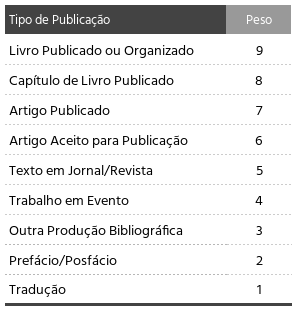
\includegraphics[width=.35\textwidth]{heuristics.png}
\end{table}


Vale ressaltar que a heurística neste caso é relativa por haver muitos fatores que influenciam a relevância de uma publicação: artigos em certas publicações de prestígio podem valer mais que capítulos de livro, e o mesmo pode ser verdade para textos em jornais ou revistas. Da mesma maneira, publicações mais recentes podem valer mais do que publicações mais antigas, porém o contrário pode ser verdade para linhas de pesquisa na área da história, por exemplo. É possível também considerar mais do que a relevância e quantidade das publicações para descrever os laços de confiança entre pesquisadores. 

Considerando as heurísticas discutidas, é possível alcançar um fluxo de confiança mais interessante na rede modelada. O conceito de agregação e dissipação de confiança pode seguir a ideia do algoritmo PageRank aplicando-se um algoritmo para o cálculo da centralidade dos nodos (Equação~\ref{eqn:centrality}). No caso, a relevância das publicações e a quantidade de colaborações devem ser levadas em consideração na distribuição de confiança. Ao incorporar o número e a relevância das publicações como um peso para as arestas da rede, é reintroduzido o conceito de considerar a confiança da comunidade nos colaboradores que depositaram confiança em determinado autor através de publicações em  conjunto para o cálculo da confiança estimada de tal autor. Assim, é possível chegar em um fluxo de confiança apurado levando em conta informações sobre obras e autores que são relevantes para considerar a confiança compartilhada entre os membros da rede.

Na Tabela~\ref{tab:centrality} são apresentados os diferentes valores computados para a centralidade de cada nodo aplicando-se a Equação~\ref{eqn:centrality} na rede exemplificada na Figura~\ref{fig:network}, variando o parâmetro $\alpha$. No caso, as recomendações seriam ordenadas do maior para o menor valor computado. Para $\alpha = 0$ a centralidade de cada pesquisador seria igual ao número de colaborações, aumentando-se $\alpha$ é atribuída maior importância para a heurística de relevância das publicações.

{\tiny
  \begin{table}[ht]
    \caption{Centralidade}
    \label{tab:centrality}
    \centering
    \begin{tabular}{|lcccc|}
      \hline
      \rowcolor[HTML]{343434} 
      \multicolumn{1}{|c}{\cellcolor[HTML]{343434}{\color[HTML]{FFFFFF} }}                       & \multicolumn{4}{c|}{\cellcolor[HTML]{343434}{\color[HTML]{FFFFFF} $C_D ^{w \alpha} (i)$}}                                              \\
      \rowcolor[HTML]{656565} 
      \multicolumn{1}{|c}{\multirow{-2}{*}{\cellcolor[HTML]{343434}{\color[HTML]{FFFFFF} Nodo}}} & {\color[HTML]{FFFFFF} $\alpha := 0.00$} & {\color[HTML]{FFFFFF} $\alpha := 0.50$} & {\color[HTML]{FFFFFF} $\alpha := 1.00$} & {\color[HTML]{FFFFFF} $\alpha := 1.50$} \\
      \multicolumn{1}{|l|}{A}                                                                    & 3.00                        & 5.47                        & 10.00                       & 18.25                       \\
      \multicolumn{1}{|l|}{B}                                                                    & 3.00                        & 5.74                        & 11.00                       & 21.06                       \\
      \multicolumn{1}{|l|}{C}                                                                    & 2.00                        & 3.16                        & 5.00                        & 7.90                        \\
      \multicolumn{1}{|l|}{D}                                                                    & 2.00                        & 5.09                        & 13.00                       & 33.00                       \\
      \multicolumn{1}{|l|}{E}                                                                    & 2.00                        & 5.09                        & 13.00                       & 33.00                       \\ \hline
    \end{tabular}
  \end{table}  
  }


A centralidade do pesquisador, ponderada pelo número de colaborações e suas relevâncias se mostra em teoria uma forte métrica de confiança global. O cálculo de confiança local, porém, oferece uma estimativa da \textbf{confiança subjetiva} de um usuário em relação aos membros da rede. Outra métrica valiosa neste contexto é a distância entre os pesquisadores, isto é, identificar \textbf{amigos de amigos} e pesquisadores próximos na rede é uma maneira de promover a colaboração entre pesquisadores: pesquisadores próximos na rede podem encontrar mais facilidade para realizar colaborações. Para tal, a relevância e quantidade de colaborações (pesos das arestas - confiança) deve ser um fator positivo e o número de nodos intermediários entre os autores um fator negativo (maior distância).

O conceito de distância (discutido na Seção~\ref{sect:analysis} e ilustrado na Equação~\ref{eqn:distance}), aplicado à rede de colaborações, significa que a distância entre os pesquisadores levará em consideração o nível de confiança das conexões bem como o número de pesquisadores intermediários. Para $\alpha < 1$, caminhos com maior número de intermediários são considerados mais distantes, enquanto $\alpha > 1$ vai considerar mais importante a força das relações de confiança, atribuindo menores distâncias para caminhos onde há fortes relações de confiança entre os pesquisadores, podendo estes ter mais intermediários \cite{opsahl2010node}. Na Tabela~\ref{tab:distances} são apresentadas as distâncias calculadas entre os pesquisadores A e B, conforme a rede exemplificada na Figura~\ref{fig:network}. As recomendações seriam ordenadas da menor para a maior distância.

{\tiny
  \begin{table}[ht]
    \caption{Distâncias}
    \label{tab:distances}
    \centering
    \begin{tabular}{|lcccc|}
      \hline
      \rowcolor[HTML]{343434} 
      \multicolumn{1}{|c}{\cellcolor[HTML]{343434}{\color[HTML]{FFFFFF} }}                       & \multicolumn{4}{c|}{\cellcolor[HTML]{343434}{\color[HTML]{FFFFFF} $ d^{w\alpha}(i, j) $}}                                               \\
      \rowcolor[HTML]{656565} 
      \multicolumn{1}{|c}{\multirow{-2}{*}{\cellcolor[HTML]{343434}{\color[HTML]{FFFFFF} Caminho}}} & {\color[HTML]{EFEFEF} $ \alpha := 0.00 $} & {\color[HTML]{EFEFEF} $ \alpha := 0.50 $} & {\color[HTML]{EFEFEF} $ \alpha := 1.00 $} & {\color[HTML]{EFEFEF} $ \alpha := 1.50 $} \\ \cline{1-1}
      \multicolumn{1}{|l|}{\{A, B\}}                                                             & 1.00                        & 0.81                        & 0.50                        & 0.35                        \\
      \multicolumn{1}{|l|}{\{A, C, B\}}                                                          & 2.00                        & 1.53                        & 0.83                        & 0.54                        \\
      \multicolumn{1}{|l|}{\{A, D, E, B\}}                                                       & 3.00                        & 1.72                        & 0.47                        & 0.19                        \\ \hline
    \end{tabular}
  \end{table}  
  }


\subsection{Pré-seleção de Recomendações} \label{sect:pre-selection}

Com as métricas de confiança propostas, é possível estabelecer níveis de confiança da comunidade, uma rede subjetiva do pesquisador alvo ou distâncias ponderadas por confiança e usar as predições para oferecer sugestões de colaboradores para cada membro da rede em diferentes contextos. Todavia, confiança apenas pode não ser suficiente para recomendações de qualidade. Considerar também a linha de pesquisa do pesquisador no momento e os perfis dos potenciais colaboradores pode aumentar a qualidade das recomendações: mesmo que a confiança em um pesquisador seja alta, a sugestão de colaboração pode não fazer sentido caso as linhas de pesquisa não se encaixem.

Para aprimorar as recomendações, é proposta uma pré-seleção dos itens utilizando um método baseado em conteúdo. A técnica consiste no cálculo de correspondência de palavras chave em um modelo de espaço vetorial (MEV), visto que esta é a mais comum em sistemas de recomendação baseados em conteúdo \cite{ricci2011introduction}. O perfil do pesquisador é representado por um vetor em um espaço \textit{n-dimensional}: $d_j = {w_{1,j}, w_{2,j}, \dots ,d_{n,j}}$, no qual $w_{i,j}$ representa o quanto o termo $i$ é relevante dentro do trabalho do pesquisador $j$. Pode-se pensar em uma matriz na qual as linhas são pesquisadores, conforme descrito e as colunas representam os termos-chave extraídos do universo das publicações (\textit{corpus}), removendo palavras vazias - “ou”, “de”, “para” \dots - tanto em português quanto em inglês.Tal matriz é construída por meio da técnica de vetorização \textit{TF-IDF}, na qual considera-se termos importantes aqueles que aparecem com frequência relacionados á um item específico e com menor frequência nos outros itens do \textit{corpus} \cite{pazzani2007content}. 

A partir disso, é preciso computar a semelhança entre termos. Para tal, a proposta é o uso da similaridade de cossenos por ser a técnica mais comumente aplicada \cite{ricci2011introduction}. Para a pré-seleção dos itens, a proposta é basear-se em uma \textit{query} que representa o trabalho sendo desenvolvido pelo pesquisador no presente.

\subsection{Arquitetura} \label{sect:arch}

Até este ponto do texto foram descritas técnicas que podem ser usadas para a computação de confiança entre membros de uma comunidade, resultando em vetores de confiança global e local, bem como distâncias ponderadas por confiança. Também foi discutida a possibilidade de aprimorar recomendações baseadas em confiança usando o conteúdo dos itens disponíveis. Agora, detalha-se de como é possível combinar as metodologias descritas para obter um resultado.

\begin{figure}[ht]
    \centering
    \includegraphics[width=.78\textwidth]{SR-arch.png}
    \caption{Arquitetura do Sistema de Recomendação proposto.}
    \label{fig:sr-arch}
\end{figure}

Em \cite{massa2004trust}, é sugerida uma arquitetura de SR combinando filtragem colaborativa e método baseado em confiança. O sistema é descrito em módulos substituíveis e, portanto, pode ser usado para combinar os métodos baseado em conteúdo e em confiança. Basicamente, conforme apresentado na Figura~\ref{fig:sr-arch}, a saída do método usado para pré-seleção é usada para filtrar e ordenar as recomendações a partir das confianças computadas.

É preciso então definir um método para oferecer ao usuário uma amostra seleta com os pesquisadores mais relevantes seguindo as métricas de confiança (filtragem por confiança) a partir de uma lista de itens ordenada por similaridade de cossenos e vetores de confiança estimada. As linhas em pontilhado da Figura~\ref{fig:sr-arch} representam que os objetos são intercaláveis: pode-se usar um ou outro ou combinações. Após a pré-seleção, o custo computacional da aplicação das distâncias, por exemplo, diminui consideravelmente pois é preciso apenas computar distâncias entre o pesquisador alvo e uma amostra pequena de pesquisadores com o perfil compatível com a \textit{query}. Portanto, uma vez aplicado o método por conteúdo, pode-se  aplicar as métricas de confiança em uma amostra reduzida da rede.

\subsection{Tecnologias}

Os dados usados no trabalho são provenientes do banco de dados relacional da Plataforma Kennis (www.kennis.com.br), que extrai os dados dos currículos de pesquisadores cadastrados na Plaforma Lattes com o uso de um \textit{parser}, cuja versão inicial é descrita em \cite{prass2019parser}. Optou-se pelo uso dos dados da Plataforma Kennis e não pelos dados originais da Plataforma Lattes, pois durante o processo de \textit{parsing} dos currículos, a Plataforma Kennis faz a limpeza e o pré-processamento dos dados do website do curriculo Lattes, associando pesquisadores e suas publicações, conforme mostra a Figura \ref{fig:database}.

\begin{figure}[ht]
    \centering
    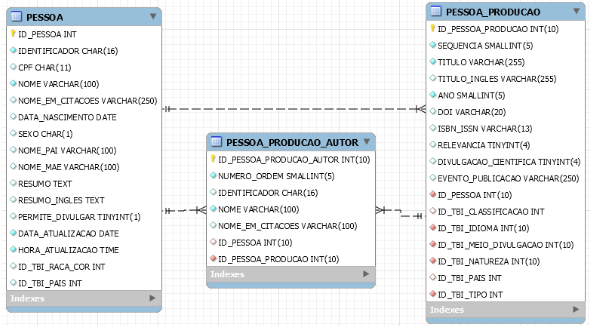
\includegraphics[width=.55\textwidth]{database.png}
    \caption{Tabelas Pessoa, Produção e associativa \cite{prass2019parser}.}\label{fig:database}
\end{figure}
 
A partir do banco, foi possível construir uma base de conhecimento focada especificamente no objetivo do trabalho. Foi gerado a partir dos dados da Kennis um arquivo com dados como o titulo da obra, a ID de seu autor, seu tipo (os possíveis tipos de obras são ilustrados na Tabela~\ref{tab:relavancy}), palavras chaves e o contexto de sua publicação. Os dados exportados da plataforma Kennis resultaram em um arquivo \textit{csv - comma separated value} com 16793 linhas, cada uma representando uma publicação cadastrada por seu autor.

Foi usada a linguagem Python que possui riqueza de recursos para trabalhos relacionados a manipulação de dados e computação numérica. A biblioteca pandas facilita a descoberta de conhecimento em bancos de dados, oferecendo objetos que encapsulam uma base de dados e ajudam na sua manipulação. Aliado com a biblioteca \textit{scikit-learn} que implementa diversos algoritmos usados na mineração de dados e computação científica (como vetorização TF-IDF e o algoritmo de clusterização MeanShift \cite{scikit-learn}), também foi utilizada a biblioteca numpy para computação numérica. O pacote \textit{NetworkX} oferece um ambiente de programação (API) para a criação, manipulação e estudo de redes complexas, com implementação de algoritmos de análise de grafo capazes de tratar grandes \textit{datasets}, devido ao uso de linguagens como o C++ na implementação dos algoritmos \cite{networkx2008}. A distribuição \textit{Anaconda} funciona como um gerenciador de pacotes e ambientes da linguagem Python e por padrão oferece todas as bibliotecas citadas, além da interface \textit{jupyter}, que facilita a exploração de dados por via de uma interface gráfica acessível via navegador.

Para a execução do código, foram usados diversos serviços de computação em nuvem variando nas seguintes características: hardware, preço, disponibilidade de tempo e facilidade de uso. A plataforma \textit{datalore} não possui limite de uso e é capaz de proporcionar um ambiente anaconda para usuário cadastrados depois de poucos cliques, de graça. Porém, possuía apenas instâncias com 4GB de memória RAM e uma CPU de 2 \textit{cores} e não está disponível a todo o tempo, apresentando quedas do servidor que embora raras impossibilitam a total dependência da plataforma. Devido a essas limitações, a plataforma foi usada para análise exploratória dos dados e desenvolvimento dos algoritmos usando uma amostra reduzida dos dados. Para computações custosas usando a base completa, foi usada a plataforma \textit{salamander.ai}, que oferece facilidade semelhante a da plataforma \textit{datalore} para o \textit{deploy} de instâncias prontas para o uso. A plataforma não possui modalidades de graça e é preciso adicionar créditos, que são deduzidos da conta do usuário conforme o tempo de uso e ao hardware selecionado. Foi usada uma instância de 36 núcleos otimizados para computação e 72 gigabytes de memória RAM, ao custo de 93 centavos de dólar por hora. Por fim, o \textit{Google cloud platform} (GCP) oferece opções de hardware para seleção do usuário de até 96 núcleos, com um crédito inicial de 300 dólares de bônus. Porém não oferece nenhuma configuração prévia, exigindo o usuário fazer a configuração do ambiente. No GCP foi usado 16 núcleos de CP otimizados para computação e 32 gigabytes de RAM, pois observou-se que o uso de CPU era limitado pela quantidade de RAM disponível.

\section{Resultados e Discussões}

Nesta seção, buscou-se apresentar alguns resultados relevantes e já discuti-los, para facilitar o entendimento da proposta e dos próprios resultados.

\subsection{Pré-Processamento}

Os dados originalmente contém 169 autores e 15821 títulos de obra distintos. É importante notar que os títulos distintos não representam publicações distintas, pois é possível que dois pesquisadores cadastrem a mesma publicação com títulos levemente diferentes (devido a erros de caligrafia, supressão de artigos, distinções de acentuação e de letras maiúsculas ou minúsculas), o que pode causar com que a mesma publicação apareça diversas vezes com pequenas variações de título. Por isso, na fase de pré-processamento se fez necessário agrupar as publicações em comum cadastradas por pesquisadores distintos.

Foi gerada uma matriz TF-IDF usando a classe \textit{TfidfVectorizer} de \textit{scikit-learn}, que resultou em uma tabela com todos os termos que apareciam nos títulos dos artigos, entretanto, foi necessário excluir as palavras vazias (artigos, preposições e outros). Essa matriz tinha as 17 mil linhas da base original, mas 20 mil colunas, referentes aos termos dos títulos. O valor da linha coluna era a importância do termo para o artigo.

Para agrupar as publicações foi usado o algoritmo \textit{MeanShift}, conforme exposto pela Seção~\ref{sect:analysis}, na matriz TF-IDF dos títulos das obras. Foram feitos testes com o parâmetro \textit{bandwidth} variando de $0.3$ até $1.0$, procurando um valor no qual os \textit{clusters} resultantes correspondem a publicações em comum cadastradas por pesquisadores distintos. Notavelmente, valores mais altos acabaram por agrupar títulos diferentes em um único \textit{cluster}, efetivamente resultando em falsos positivos. Observou-se que o valor $0.3$ resultou em \textit{clusters} nos quais os títulos eram efetivamente os mesmos, diferindo principalmente em detalhes como acentuação ou supressão de artigos. Depois da clusterização, foram filtrados os dados para remover as publicações que não foram agrupadas em nenhum \textit{cluster} e \textit{clusters} nos quais todas as publicações são pertencentes a um mesmo autor, pois representam arestas da rede que não conectam dois autores.

\begin{figure}[ht]
\centering
  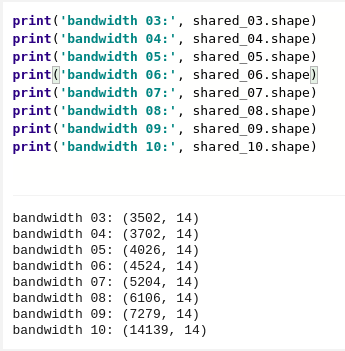
\includegraphics[width=.35\textwidth]{shared-size.png}
  \caption{Numero de linhas, colunas do arquivo csv depois da filtragem}
  \label{fig:numeroCluster}
\end{figure}

A Figura~\ref{fig:cluster03} exemplifica um \textit{cluster} obtido usando um \textit{bandwidth} de $0.3$. Pode-se notar que embora tenha pequenas variações no título, a publicação de ID (\textit{pubid} na tabela) $26$ trata-se de um trabalho publicado em evento no ano 2015 cadastrado pelos autores $6, 9, 70 \And 128$ (coluna $authid$). A Figura~\ref{fig:numeroCluster} mostra a quantidade de linhas dos dados depois da filtragem. Por exemplo, o cluster \textit{bandwidth} $03$ possui 3502 publicações e 14 colunas após a filtragem. A biblioteca Pandas foi usada para a filtragem dos dados. Foi definida uma função $not\_single$, que retorna as publicações que não são únicas, e tambem uma função $shared\_pubs$, que aplica $not\_single$ aos dados e permite somente os \textit{clusters} com mais de uma publicação.

\begin{figure}[ht]
\centering
  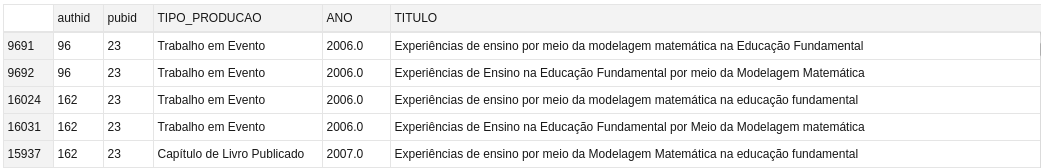
\includegraphics[width=1\textwidth]{shared-03-cluster.png}
  \caption{Exemplo de um cluster com bandwidth 0.3.}
  \label{fig:cluster03}
\end{figure}

\subsection{Estimativa de confiança}

Foi usado o tipo \textit{DiGraph} presente em \textit{NetworkX} para a modelagem da rede de confiança. O tipo representa um grafo não-direcionado com a possibilidade de múltiplas arestas entre dois nodos. Assim, para cada publicação em comum entre dois pesquisadores, foi adicionada uma aresta entre eles com o peso equivalente aos das heurísticas apresentadas na Tabela~\ref{tab:relavancy}. Para a atribuição da heurística na formação do grafo, os dados pré-processados foram lidos de um arquivo CSV resultante da fase de pre-processamento, e então foi adicionada uma coluna numérica com o valor correspondente ao tipo de cada publicação. 

Foram então definidas funções para a geração da rede de confiança. Destaca-se a função \textit{edge} que retorna as publicações em comum e foi usada para popular o grafo da rede de confiança.
A Figura~\ref{fig:trust-estimative-code-centrality-distances} mostra as funções que calculam as equações de distância e centralidade apresentadas na seção de revisão bibliográfica, a função $path\_length$ implementa a Equação~\ref{eqn:distance} e a função $degree\_centrality$ implementa a Equação~\ref{eqn:centrality}.

\begin{figure}[ht]
  \centering
  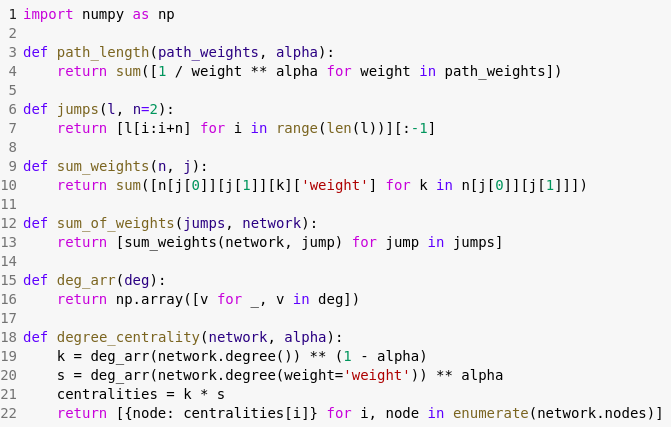
\includegraphics[width=.7\textwidth]{trustest_code_c.png}
  \caption{Estimativa de confiança via centralidade e distancias.}
  \label{fig:trust-estimative-code-centrality-distances}
\end{figure}

A Figura~\ref{fig:trust-estimative-results}~(a) apresenta o resultado das estimativas de confiança por distância entre os pesquisadores $u_1 := 14  \dots u_n := 40$. A esquerda observa-se uma lista representando o caminho percorrido e a direita o valor da distancia. Pode-se observar que embora a biblioteca \textit{NetworkX} gere caminhos repetidos, eles possuem o mesmo valor para a distância pois o algoritmo leva em consideração o numero de arestas entre os nodos \cite{opsahl2010node}. Por apresentar um número muito grande de caminhos com muitos intermediários no grafo, foi necessário realizar uma poda (parâmetro \textit{cutoff}). Na Figura~\ref{fig:trust-estimative-results}~(b) observa-se a computação das as centralidades de cada pesquisador, ou seja, a estimativa de confiança global. Cada item da lista representa um par $\{chave: valor\}$, sendo a chave a ID do pesquisador e o valor a sua centralidade. Destaca-se que o tempo de processamento desse processo foi menor que o processo de cálculo de distâncias, e também que a métrica centralidade pode ser re-aproveitada para múltiplas recomendações, enquanto as distancias devem ser calculadas para cada par de pesquisadores.

\begin{figure}
    \centering
    \hfill
    \subfigure[Distancias]{\includegraphics[width=8.5cm]{trustest_distances.png}}
    \hfill
    \subfigure[Centralidade]{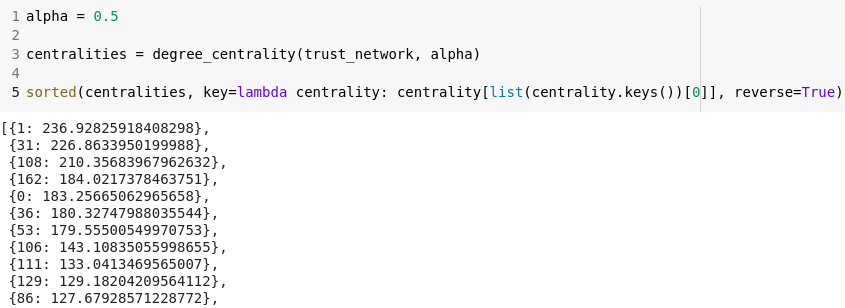
\includegraphics[width=4cm]{trustest_code_d.png}}
    \hfill
    \caption{Estimativas de confiança com $\alpha := 0.5$}
    \label{fig:trust-estimative-results}
\end{figure}

As métricas apresentadas podem então ser aplicadas ao resultado de uma pre-seleção qualquer, tal como a apresentada na Figura~\ref{fig:sr-arch}, para aumentar o escopo das recomendações obtidas com a dimensão confiança. Por exemplo, sendo o resultado da recomendação baseada em conteúdo uma lista ordenada de pesquisadores, pode-se re-ordenar a lista utilizando uma das métricas sugeridas, ou uma combinação delas.

\begin{figure}[ht]
\centering
  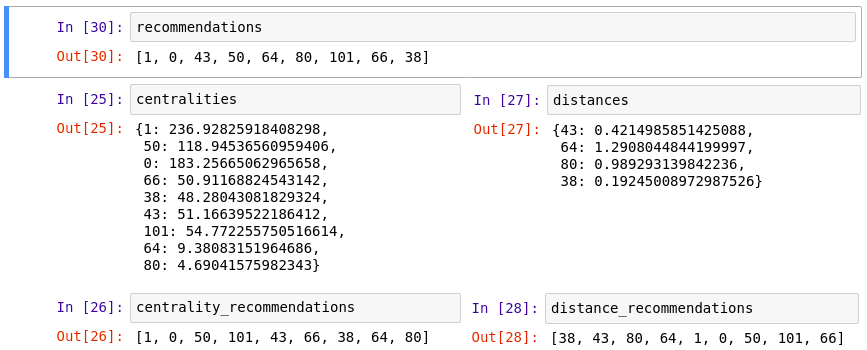
\includegraphics[width=1\textwidth]{peer-recommendations.png}
  \caption{Exemplo de Recomendações.}
  \label{fig:peer-recommendations}
\end{figure}

Para ilustrar a arquitetura discutida na Seção~\ref{sect:arch}, definiu-se uma função, que recebe uma ID de pesquisador e retorna um vetor com as IDs dos pesquisadores com perfis mais semelhantes por similaridade de cossenos conforme discutido na Seção~\ref{sect:pre-selection}. Na célula $30$ da Figura~\ref{fig:peer-recommendations}, o vetor $recommendations$ representa a pré-seleção baseada em conteúdo para o pesquisador de $ID:=1$ (como o próprio pesquisador não é excluído para a seleção dos mais semelhantes, nota-se que ele é o primeiro perfil sugerido, validando a recomendação baseada em conteúdo). As células $25 \& 26$ respectivamente representam os valores da centralidade da pré-seleção ($centralities$) e a lista re-ordenada de recomendações ($centrality\_recommendations$), baseando-se em centralidade e as células $27 \& 28$ mostram as distâncias entre o pesquisador 1 e os pesquisadores da pré-seleção para os quais existem caminhos na rede ($distances$), bem como a lista ordenada por distâncias ($distance\_recommendations$).

\section{Conclusões}

Neste trabalho buscou-se apresentar sistemas de recomendação para promover a colaboração entre membros de uma comunidade de pesquisadores. Foram discutidos conceito de Sistema de Recomendação, as técnicas mais utilizadas e uma tendência mais recente de recomendações baseadas em confiança. Sugeriu-se um modelo de rede de confiança na qual pesquisadores são conectados por publicações em conjunto, considerado um voto de confiança. Também foram discutidas três métricas de propagação e agregação de confiança  na rede, usando conceitos do algoritmo PageRank \cite{page1999pagerank} e de métricas de centralidade e distância entre nodos em grafos não-direcionados ponderados \cite{opsahl2010node}.

A partir disso, foi proposta a recomendação por meio da pré-seleção de perfis baseada em conteúdo, seguida de filtragem dos perfis via estimativas de confiança, obedecendo a arquitetura proposta por Massa e Avesani \cite{massa2004trust} para um SR híbrido utilizando o método baseado em conteúdo. 

Com relação aos resultados obtidos, destaca-se que a recomendação baseada em centralidades se mostrou mais eficaz computacionalmente, pois os valores são calculados com rapidez e podem ser reutilizados, enquanto as recomendações baseadas em distância devem ser calculadas par-a-par e são computacionalmente complexas pois dependem de uma busca em grafo por (todos os) caminhos entre dois nodos, porém são capazes de achar amigos de amigos, o que pode influenciar a facilidade da colaboração. Nos resultados da Figura~\ref{fig:peer-recommendations} observa-se que para o pesquisador 1 (que possui a maior centralidade entre todos os pesquisadores dos dados) foi possível achar distâncias para apenas 4 das 9 recomendações da pré-seleção. Sugere-se então a combinação das duas métricas aplicando a centralidade aos perfis para os quais não é possível aplicar a distância.

É possível estender o trabalho proposto pensando em melhores heurísticas para a relevância das publicações. Também sugere-se como trabalho futuro o processo de validação do Sistema de Recomendação. Em \cite{shani2011evaluating}, os autores sugerem que é importante considerar o contexto da aplicação de cada SR, pois como os objetivos de diferentes sistemas variam, é natural que variem também as métricas de validação. Como o principal fator de sucesso do SR  proposto é a promoção da colaboração entre os pesquisadores da rede, a métrica mais completa para a validação do sistema é subjetiva ao usuário.

\bibliographystyle{sbc}
\bibliography{sbc-template}

\end{document}